\documentclass[conference]{IEEEtran}

\usepackage[T1]{fontenc}
\usepackage{amsmath,amssymb}
\usepackage{graphicx}
\usepackage{url}

\graphicspath{{figures/}}
\newcommand{\Samples}{2275}
\newcommand{\RequestedTime}{26.000}
\newcommand{\WallTime}{26.010}
\newcommand{\TimingError}{0.010}
\newcommand{\TimingPercent}{0.040}
\newcommand{\PlanningTime}{0.053}
\newcommand{\Iterations}{119}
\newcommand{\TreeNodes}{55}
\newcommand{\RawLength}{13.194}
\newcommand{\SmoothLength}{11.679}
\newcommand{\MinimumTime}{23.358}
\newcommand{\RmseX}{0.0309}
\newcommand{\RmseY}{0.0413}
\newcommand{\RmseZ}{0.0025}
\newcommand{\RmseVector}{0.0517}
\newcommand{\MaxX}{0.1166}
\newcommand{\MaxY}{0.1434}
\newcommand{\MaxZ}{0.0092}
\newcommand{\MaxXY}{0.1516}
\newcommand{\FinalError}{0.0228}
\newcommand{\FinalYaw}{0.000088}
\newcommand{\PeakReferenceSpeed}{0.674}
\newcommand{\PeakMeasuredSpeed}{0.822}


\title{Continuous Time-Parameterized RRT Navigation for a Simulated Quadrotor in ROS~2 and Gazebo}

\author{\IEEEauthorblockN{Sarah Daniela Vásquez Melgarejo}
\IEEEauthorblockA{Robotics Practice 4\\
ROS~2 Humble and Gazebo Classic}}

\begin{document}

\maketitle

\begin{abstract}
This paper presents a collision-aware navigation system for a simulated
quadrotor that receives an arbitrary Cartesian destination and desired flight
time through a ROS~2 action. A rapidly-exploring random tree (RRT) is built on
an inflated occupancy representation of a Gazebo world. Line-of-sight
shortcuts and collision-checked quadratic B\'ezier arcs convert the resulting
polyline into a smooth geometric path. The path is parameterized by arc length
and traversed with one global cubic timing law, thereby preserving velocity
through intermediate points and imposing zero velocity only at the initial and
final configurations. Feed-forward velocity and proportional feedback provide
trajectory tracking, while an explicit feasibility rule of two seconds per
meter prevents physically unrealistic timing requests. In a representative
obstacle-avoidance experiment, the smoothed route measured \SmoothLength~m and
was completed in \WallTime~s for a requested \RequestedTime~s. The final
position error was \FinalError~m, the maximum transient horizontal error was
\MaxXY~m, and no Gazebo contact was detected. The experiment demonstrates that
the planner, smoother, time parameterization, and controller operate as a
single action-driven navigation pipeline without stopping at intermediate
waypoints.
\end{abstract}

\begin{IEEEkeywords}
RRT, quadrotor navigation, trajectory smoothing, time parameterization,
ROS~2, Gazebo, collision avoidance.
\end{IEEEkeywords}

\section{Introduction}

Sampling-based planning is useful when the free configuration space has a
geometry for which a direct start-to-goal segment is obstructed. An RRT rapidly
explores that space by extending a tree toward random samples
\cite{lavalle1998,lavalle2006}.
Nevertheless, a collision-free RRT polyline is not by itself a suitable flight
reference: it contains unnecessary vertices, abrupt changes in direction, and
no information about when each part of the route must be traversed. Treating
every vertex as an independent position objective further causes the vehicle to
brake and settle repeatedly, increasing the total time and producing visibly
discontinuous motion.

The objective of this work is to navigate the \texttt{simple\_drone} model to
any collision-free coordinate supplied through the existing
\texttt{/pidcontrol} action. Planning begins only after a goal is received and
uses the current vehicle pose as the tree root. Thus, consecutive destinations
can be commanded without restarting Gazebo. The implementation satisfies five
requirements: construction of an obstacle world; an occupancy representation
of free and occupied space; collision-free RRT planning with smoothing;
generation of a time-parameterized trajectory; and execution of that trajectory
within a feasible user-specified duration.

The principal design choice is to separate the geometric path from its timing.
Intermediate RRT points constrain the route around obstacles, but they are not
control objectives at which the quadrotor must settle. One differentiable
progress law spans the complete route, and a feed-forward term carries the
vehicle through its interior. A strict final tolerance is evaluated only when
the requested time expires. This formulation directly addresses both the
stopping behavior of waypoint-by-waypoint control and the ambiguity between
``arrival time'' and an additional settling interval.

The analytical expressions used below are distinguished from parameters chosen
for this implementation. The RRT, configuration-space inflation, B\'ezier
representation, cubic time scaling, coordinate transformations, proportional
velocity control, and RMSE definition follow established references. In
contrast, the numerical gains, safety margins, terminal tolerances, and the
two-second-per-meter feasibility threshold were selected and validated
experimentally for the simulated vehicle; they are not asserted as universal
results.

\section{World Representation and Problem Formulation}

Let the translational state be
$\mathbf{p}=[x\ y\ z]^\mathsf{T}$ and let $\psi$ denote yaw. Each action goal
specifies
\begin{equation}
  \mathbf{g}=[x_d\ y_d\ z_d\ \psi_d\ T]^\mathsf{T},
\end{equation}
where $T$ is the desired wall-clock execution time. The planning problem is to
find a planar curve $\boldsymbol{\gamma}:[0,L_{xy}]\rightarrow\mathcal{C}_{free}$
from the current $(x,y)$ position to $(x_d,y_d)$, then construct a spatial
reference $\mathbf{p}_d(t)$ over $t\in[0,T]$. Obstacles are 5~m high and the
accepted altitude range remains below their top surfaces; consequently, a
collision-free horizontal path is required rather than an overflight.

The Gazebo world covers $[-8,8]\times[-8,8]$~m and contains the three rectangular
obstacles in Table~\ref{tab:obstacles}. The same YAML description generates the
world and the occupancy grid, preventing a separate hand-coded map from
silently diverging from the simulation. At run time, the node also verifies the
name and pose of every obstacle in Gazebo before commanding motion.

\begin{table}[t]
\caption{Obstacle Geometry in the Gazebo World}
\label{tab:obstacles}
\centering
\begin{tabular}{lrrrr}
\hline
Obstacle & $x$ (m) & $y$ (m) & width (m) & depth (m)\\
\hline
\texttt{wall\_middle} & 3.0 & 0.0 & 1.0 & 6.0\\
\texttt{block\_left}  & $-3.0$ & 2.0 & 2.0 & 2.0\\
\texttt{block\_lower} & $-2.0$ & $-4.0$ & 2.0 & 1.5\\
\hline
\end{tabular}
\end{table}

The binary occupancy grid has a 0.1~m resolution. For planning, each obstacle
and the world boundary are inflated by
\begin{equation}
  \rho_p=r_d+m_p=0.40+0.50=0.90~\text{m},
  \label{eq:inflation}
\end{equation}
which is the Minkowski sum of the rectangular obstacle with a circular vehicle
footprint and planning margin, following the standard construction of
configuration-space obstacles \cite[Ch.~4]{lavalle2006}. A candidate RRT edge is checked as a full line
segment against occupied cell boxes using slab intervals. This rejects a
crossing even when neither edge endpoint lies inside the obstacle. A separate,
less conservative physical envelope uses $r_d+0.15=0.55$~m; entry into this
region or a Gazebo contact terminates execution.

\section{Planning and Continuous Trajectory Generation}

\subsection{Rapidly-Exploring Random Tree}

At each iteration, the planner samples the destination with probability
$p_g=0.15$ and otherwise samples uniformly from free space, following the RRT
construction in \cite{lavalle1998} and \cite[Sec.~5.5]{lavalle2006}. Given a random
sample $\mathbf{q}_{rand}$, the Euclidean nearest tree vertex
$\mathbf{q}_{near}$ is extended by
\begin{equation}
 \mathbf{q}_{new}=\mathbf{q}_{near}+
 \min\!\left(1,\frac{\eta}{\lVert\mathbf{q}_{rand}-\mathbf{q}_{near}\rVert_2}\right)
 (\mathbf{q}_{rand}-\mathbf{q}_{near}),
 \label{eq:steer}
\end{equation}
where the step size is $\eta=1.0$~m. The new edge is inserted only if its entire
segment is collision-free. A direct goal connection is attempted when a vertex
is within 0.8~m of the destination and must pass the same segment test. Parent
pointers reconstruct the route. The random seed is stored with the evidence so
that the experiment is repeatable; reaching the 10,000-iteration limit is
reported as planning failure rather than as proof that a path does not exist.

\subsection{Collision-Checked Smoothing}

The raw route first undergoes up to 200 seeded shortcut attempts. For two
nonconsecutive vertices $\mathbf{P}_i$ and $\mathbf{P}_j$, the intervening
vertices are deleted only when the segment $\overline{\mathbf{P}_i\mathbf{P}_j}$
is collision-free. This process reduced the representative path to four
waypoints: the two endpoints and two intermediate points that carry the route
below the central wall.

The remaining corners are rounded with quadratic B\'ezier curves in Bernstein
form \cite[Chs.~4--5]{farin2002},
\begin{equation}
 \mathbf{B}(v)=(1-v)^2\mathbf{P}_0+2(1-v)v\mathbf{P}_c+v^2\mathbf{P}_1,
 \quad v\in[0,1],
 \label{eq:bezier}
\end{equation}
where $\mathbf{P}_c$ is the original corner and $\mathbf{P}_0,\mathbf{P}_1$
are trimmed points on its incident segments. The nominal trim distance is 2~m
and is reduced adaptively if necessary. Twenty samples per corner and every
connecting edge are validated against the inflated occupancy map. Therefore,
smoothing cannot replace a safe RRT segment by an unchecked curve. The
underlying B\'ezier arc has continuous tangent direction, and its dense sampled
representation approximates that property for execution. In the reported run,
the rounded path contains 44 samples and has length
$L_{xy}=\SmoothLength$~m.

\subsection{Arc-Length and Global Time Parameterization}

Let $s\in[0,L_{xy}]$ be cumulative arc length along the dense smooth curve
\cite[Ch.~11]{farin2002}.
Linear interpolation in $s$ defines $\boldsymbol{\gamma}(s)$ and its unit
tangent $\boldsymbol{\tau}(s)$. Following the path/time separation and
third-order endpoint-rest time scaling described by Lynch and Park
\cite[Ch.~9]{lynchpark2017}, a normalized elapsed time $u$ and global cubic
progress $\sigma$ are defined by
\begin{align}
 u(t)&=\operatorname{clip}(t/T,0,1),\\
 \sigma(u)&=3u^2-2u^3,\label{eq:cubic}\\
 \dot{\sigma}(t)&=\frac{6u(1-u)}{T}.
\end{align}
The complete position and feed-forward velocity references are
\begin{align}
 \mathbf{p}_d(t)&=
 \begin{bmatrix}
 \boldsymbol{\gamma}\!\left(L_{xy}\sigma\right)\\
 z_0+(z_d-z_0)\sigma
 \end{bmatrix},\label{eq:positionref}\\
 \dot{\mathbf{p}}_d(t)&=
 \begin{bmatrix}
 \boldsymbol{\tau}\!\left(L_{xy}\sigma\right)L_{xy}\dot{\sigma}\\
 (z_d-z_0)\dot{\sigma}
 \end{bmatrix}.
 \label{eq:velocityref}
\end{align}
Because $\dot{\sigma}=0$ only at $u=0$ and $u=1$, the reference does not stop at
an intermediate RRT or B\'ezier point. The B\'ezier rounding changes direction
continuously at a corner, while arc-length parameterization prevents vertex
density from determining the local traversal time.

Because the same $\sigma$ advances the horizontal arc and altitude, the
Euclidean combination used in this implementation gives the three-dimensional
route estimate
\begin{equation}
 L=\sqrt{L_{xy}^{2}+(z_d-z_0)^2}.
 \label{eq:spatiallength}
\end{equation}
The following feasibility rule is an empirical design criterion for the
simulated vehicle, rather than a bound taken from the literature:
\begin{equation}
 T\geq T_{min}=2L,
 \label{eq:mintime}
\end{equation}
with $T$ in seconds and $L$ in meters. Requests below this limit are rejected
before motion and the required minimum is printed. Since the maximum of
$6u(1-u)$ is $1.5$, the theoretical peak translational reference speed is
\begin{equation}
 v_{d,max}=\frac{1.5L}{T}.
 \label{eq:peakvelocity}
\end{equation}
Consequently, (\ref{eq:mintime}) limits this peak to approximately 0.75~m/s.
This explains why a request such as 1~m in 1~s is not a suitable timing target:
the cubic law must both accelerate and decelerate inside that second, and the
simulated vehicle also has attitude and velocity dynamics. The two-second-per-
meter rule provides the required control authority while maintaining a clear,
distance-dependent contract.

\section{Trajectory Tracking and Completion Criterion}

Define the world-frame position error as
$\mathbf{e}_p(t)=\mathbf{p}_d(t)-\mathbf{p}(t)$. At every control iteration,
$\mathbf{p}_d(t)$ is resampled from (\ref{eq:positionref}) at the current global
progress $\sigma(t)$. Hence, $e_x$, $e_y$, and $e_z$ are signed tracking errors
with respect to the instantaneous moving point on the smooth curve; they are
neither errors assigned to isolated waypoints nor the distance to final point B
during the complete flight. Only at $t=T$, when
$\mathbf{p}_d(T)=\mathbf{p}_B$, do these tracking errors become the terminal
goal errors used in (\ref{eq:success}). The commanded world-frame horizontal
velocity combines feed-forward and proportional correction. This is the
Cartesian adaptation of standard proportional motion control with velocity
inputs \cite[Ch.~11]{lynchpark2017},
\begin{equation}
 \mathbf{v}_{c,xy}^{W}=\dot{\mathbf{p}}_{d,xy}+K_{xy}\mathbf{e}_{p,xy},
 \qquad K_{xy}=3.5~\text{s}^{-1}.
 \label{eq:controller}
\end{equation}
It is limited to 0.9~m/s and rotated into the vehicle frame using the planar
rotation-matrix convention \cite[Ch.~3]{lynchpark2017},
\begin{equation}
 \mathbf{v}_{c,xy}^{B}=
 \begin{bmatrix}\cos\psi&\sin\psi\\-\sin\psi&\cos\psi\end{bmatrix}
 \mathbf{v}_{c,xy}^{W}.
 \label{eq:rotation}
\end{equation}
Vertical control uses
$v_{c,z}=\dot z_d+K_z e_z$, with $K_z=2.0$~s$^{-1}$ and a 0.8~m/s limit. The
yaw error avoids angular discontinuities through
\begin{equation}
 e_\psi=\operatorname{atan2}\!\left(\sin(\psi_d-\psi),
 \cos(\psi_d-\psi)\right),
\end{equation}
and $\omega_c=0.8e_\psi$ is limited to 1.0~rad/s.

Intermediate tracking errors are intentionally permitted because forcing the
vehicle to reach a small tolerance at each waypoint would impose repeated
settling phases and violate the global timing objective. Errors on the order of
10--15~cm may therefore occur around curved portions, while the inflated map
provides 0.50~m of planning clearance beyond the vehicle radius. At $t=T$, all
velocity commands are set to zero and success is determined once, using
\begin{equation}
 \lVert\mathbf{p}_d(T)-\mathbf{p}(T)\rVert_2\leq0.03~\text{m},\qquad
 |e_\psi(T)|\leq0.05~\text{rad}.
 \label{eq:success}
\end{equation}
No additional settling interval is appended. A goal outside these limits is
classified as unsuccessful. During execution, a stale pose, excessive roll or
pitch, map-envelope violation, or Gazebo contact also terminates the action
safely.

\section{Experimental Method}

The system was evaluated in ROS~2 Humble with Gazebo Classic, using the ROS~2
publish--subscribe/action architecture \cite{macenski2022} and Gazebo simulation
principles described in \cite{koenig2004}. The navigation node ran a nominal
100-Hz command loop and stored synchronized references,
poses, and errors in a CSV file using a monotonic wall clock. The measured mean
logging period was 0.01144~s (approximately 87.4~Hz), which includes ROS and
Gazebo scheduling overhead. A fixed seed of 22 was used for the reported trial.
The action command requested a flight from approximately
$(0,0,2)$~m to $(6,0,2)$~m at zero yaw in 26~s. The direct path intersects the
central wall, so successful completion requires a planned detour.
All quantities in Table~\ref{tab:results} and Figs.~\ref{fig:trajectory}--
\ref{fig:speed} correspond exclusively to this same outbound flight. Its
\texttt{results.json} file supplies the raw and smoothed planned paths in
Fig.~\ref{fig:trajectory}; the matching 2275-sample \texttt{flight.csv} supplies
the measured trajectory in Fig.~\ref{fig:trajectory}, the component errors in
Fig.~\ref{fig:errors}, and the reference and measured speeds in
Fig.~\ref{fig:speed}.

Gazebo reported zero contacts during the reported flight. In addition, 13 unit
tests exercised map loading, collision checking, planning, smoothing, and
trajectory utilities.

The CSV did not record a separate \texttt{/clock} timestamp. Consequently, all
duration values and the time axes in this paper are monotonic wall-clock
measurements; no unmeasured simulation-time duration or real-time factor is
inferred.

For $N$ logged samples, the reported component errors use the conventional RMSE
definition discussed in \cite{chai2014}, together with the maximum absolute
error:
\begin{align}
 \operatorname{RMSE}_j&=\sqrt{\frac{1}{N}\sum_{k=1}^{N}e_j[k]^2},
 \quad j\in\{x,y,z\},\label{eq:rmse}\\
 e_{j,max}&=\max_k|e_j[k]|.\label{eq:maxerror}
\end{align}
The measured speed was computed by finite differences of the recorded pose and
displayed with a 31-sample moving average to suppress differentiation noise. No
filter was applied to the position-error curves or to the numerical error
metrics.

\subsection{Reproducibility Artifact}

The ROS~2 packages, world and map configuration, launch file, tests, plotting
script, selected raw flight evidence, and complete LaTeX source are archived in
the project repository \cite{repository2026}:
\begin{center}
\url{https://github.com/SarahVasquezM/introduccion-robotica-inaoe/tree/main/practica-04-trayectorias}
\end{center}
The stored CSV and JSON files are the direct inputs used to regenerate the
figures and numerical macros in this paper.

\section{Results and Discussion}

\subsection{Planning and Spatial Tracking}

The RRT required \Iterations~iterations and \PlanningTime~s of wall time. Its
raw \RawLength-m polyline was reduced to a \SmoothLength-m collision-checked
curve, a reduction of approximately 11.5\%. Figure~\ref{fig:trajectory} compares
this geometry with the measured vehicle motion. The gray areas show occupancy
after the 0.90-m inflation in (\ref{eq:inflation}), which explains the clearance
between the plotted route and the visible obstacle boundaries in Gazebo. The
tracked path follows the lower passage and does not intersect occupied space.
In Fig.~\ref{fig:trajectory}, the dotted orange polyline is the raw RRT result,
the dashed blue curve is the smoothed collision-checked reference, and the solid
green curve is the measured motion. The displayed domain spans $-1$ to 7~m in
$x$ and $-5.5$ to 1~m in $y$, with 1-m major ticks on both axes.

\begin{figure}[t]
 \centering
 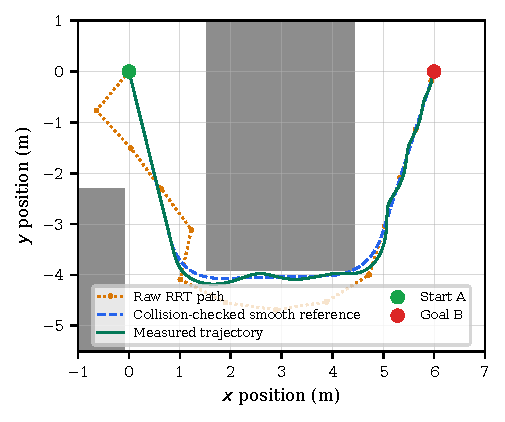
\includegraphics[width=\columnwidth]{trajectory_tracking.pdf}
 \caption{Raw RRT route, smoothed reference, and measured planar trajectory
 through the inflated occupancy map.}
 \label{fig:trajectory}
\end{figure}

Table~\ref{tab:results} summarizes the principal measurements. The final
position norm, 0.0228~m, satisfies the unchanged 0.03-m tolerance, and the yaw
error is negligible. The 0.1516-m peak horizontal error is a transient tracking
quantity rather than a missed waypoint. It occurs while the feed-forward
direction changes on the curved route and remains far below the additional
planning margin. This is the intended compromise: preserve motion and total
time through interior points, then enforce precision at the final destination.

\begin{table}[t]
\caption{Representative Obstacle-Avoidance Flight Results}
\label{tab:results}
\centering
\begin{tabular}{lr}
\hline
Metric & Measured value\\
\hline
Logged samples & \Samples\\
RRT iterations / tree nodes & \Iterations{} / \TreeNodes\\
Planning wall time & \PlanningTime~s\\
Raw / smooth route length & \RawLength{} / \SmoothLength~m\\
Minimum / requested time & \MinimumTime{} / \RequestedTime~s\\
Measured execution time & \WallTime~s\\
Timing error & \TimingError~s (\TimingPercent\%)\\
RMSE $(x,y,z)$ & (\RmseX, \RmseY, \RmseZ)~m\\
Maximum $|e_x|,|e_y|,|e_z|$ & (\MaxX, \MaxY, \MaxZ)~m\\
Maximum horizontal error norm & \MaxXY~m\\
Final position error norm & \FinalError~m\\
Final absolute yaw error & \FinalYaw~rad\\
Gazebo contact events & 0\\
\hline
\end{tabular}
\end{table}

\subsection{Error Evolution}

Figure~\ref{fig:errors} presents the three signed error components. The
horizontal components remain small along the initial straight segment, then
show bounded oscillatory transients as the path rounds the obstacle. These
curves use the instantaneous definition
$e_j(t)=p_{d,j}(t)-p_j(t)$ from (\ref{eq:controller}); consequently, each sign
change means that the measured position has crossed the moving reference in one
world-frame component. It does not indicate arrival at an RRT vertex. The
oscillations arise because the tangent of the reference rotates through the
curved detour in Fig.~\ref{fig:trajectory}, whereas the quadrotor requires a
finite attitude and velocity response to redirect its motion. The proportional
term then removes the lag and can produce a small component-wise overshoot.

This interpretation is also supported quantitatively. The maximum
$|e_x|=0.1166$~m occurs at 10.60~s and the maximum $|e_y|=0.1434$~m occurs at
15.83~s, both within the obstacle-rounding portion of the route. Their RMSE
values are 0.0309 and 0.0413~m, respectively. Altitude tracking is substantially
tighter because the reported maneuver is nearly planar: its RMSE is 0.0025~m
and maximum absolute error is 0.0092~m. The different vertical scale in the
lower panel is necessary to expose millimeter-level variation that would be
visually hidden on the $x$ and $y$ scales. Specifically, Fig.~\ref{fig:errors}
uses a common 0--26-s horizontal axis with 2-s ticks. Its $e_x$ and $e_y$ panels
span $-0.16$ to 0.16~m with 0.08-m ticks, whereas the $e_z$ panel spans
$-0.012$ to 0.012~m with 0.006-m ticks. The legend of each panel reports the
unfiltered RMSE and maximum absolute error defined in
(\ref{eq:rmse})--(\ref{eq:maxerror}).

The oscillations decay while the reference continues to advance. The nonzero
speed over the same interval in Fig.~\ref{fig:speed} and the absence of a flat
segment in Fig.~\ref{fig:trajectory} confirm continuous passage through the
intermediate geometric points. During the final cubic deceleration, the moving
reference converges to B and the controller removes the remaining lag. Near
26~s, the component errors converge to
$(-0.0113,-0.0196,-0.0024)$~m, producing the successful norm reported in
Table~\ref{tab:results}. Thus, Fig.~\ref{fig:errors} connects the continuous
tracking law in (\ref{eq:controller}) with the terminal condition in
(\ref{eq:success}).

\begin{figure}[t]
 \centering
 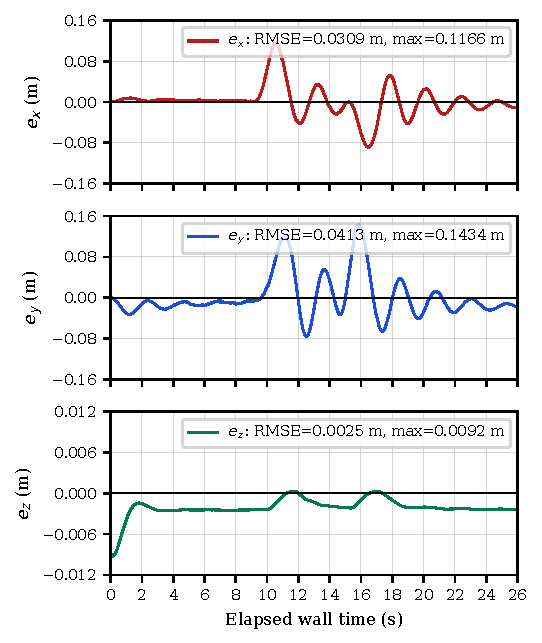
\includegraphics[width=\columnwidth]{tracking_errors_xyz.pdf}
 \caption{Signed Cartesian tracking errors relative to the instantaneous moving
 trajectory reference.}
 \label{fig:errors}
\end{figure}

\subsection{Timing and Velocity}

For $L=11.679$~m, (\ref{eq:mintime}) gives $T_{min}=23.358$~s; hence the 26-s
request is feasible. Equation~(\ref{eq:peakvelocity}) predicts a reference peak
of \PeakReferenceSpeed~m/s. Figure~\ref{fig:speed} confirms the expected cubic
acceleration and deceleration envelope. The filtered measured peak reaches
\PeakMeasuredSpeed~m/s because the proportional term in
(\ref{eq:controller}) temporarily adds corrective velocity; it remains below
the 0.9-m/s command limit. The graph spans 0--26~s with 2-s horizontal ticks and
0--0.90~m/s with 0.15-m/s vertical ticks. Its blue curve is the reference speed,
the green curve is the measured speed after a 31-sample moving average, and the
dotted horizontal line is the theoretical peak from
(\ref{eq:peakvelocity}). The elevated measured-speed intervals coincide with
the obstacle-rounding transients in Fig.~\ref{fig:errors}: the feedback term
adds velocity to recover tracking lag while the moving reference continues
along the route.

The action ended after \WallTime~s, only \TimingError~s or \TimingPercent\%
above the requested duration. This residual is approximately one control-loop
period and follows from the discrete condition that terminates on the first
iteration for which $t\geq T$. Thus, the requested duration specifies the whole
trajectory, including acceleration and deceleration, instead of being followed
by an unbounded settling phase.

\begin{figure}[t]
 \centering
 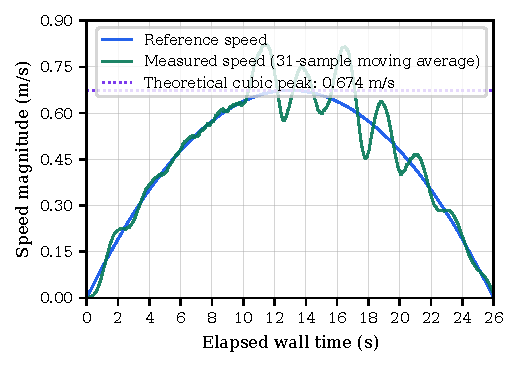
\includegraphics[width=\columnwidth]{speed_profile.pdf}
 \caption{Reference and measured translational speed during the 26-s maneuver.}
 \label{fig:speed}
\end{figure}

The experiment also illustrates why the duration cannot be interpreted without
route length. Although the endpoint displacement is 6~m, the obstacle forces an
11.679-m path. Applying two seconds per meter to the straight-line distance
would understate the required time by more than 11~s. Feasibility is therefore
evaluated after RRT planning and smoothing, using the actual route that will be
flown.

\subsection{Limitations}

The occupancy model assumes known, static, axis-aligned obstacles. Dynamic
obstacles would require online map updates and replanning. RRT is probabilistic
and the first solution is not guaranteed to be globally shortest, although the
stored seed makes each reported trial repeatable. The B\'ezier representation
provides smooth corner geometry, while the polyline arc-length interpolation
does not formally enforce higher-order dynamic limits such as jerk. Finally,
wall-clock completion can differ from $T$ by approximately one loop interval;
the measured 0.040\% timing error characterizes that implementation limit.

\section{Conclusion}

An integrated ROS~2 navigation pipeline was developed in which each action goal
triggers planning from the current pose, collision-checked smoothing, global
time parameterization, and continuous closed-loop execution. Inflated occupancy
and full-edge tests prevent the geometric route from crossing obstacles, while
contact and pose monitoring validate physical execution. Arc-length traversal
with a single cubic progress law eliminates stops at intermediate RRT points and
makes the requested time apply to the complete maneuver. The representative
Gazebo flight avoided the central wall, completed a \SmoothLength-m route within
0.010~s of its 26-s request, and reached the destination with 0.0228~m final
position error and zero contacts. The results meet the specified planning,
smoothing, temporal, and tracking requirements while retaining the original
action interface for arbitrary subsequent destinations.

\begin{thebibliography}{00}

\bibitem{lavalle1998}
S. M. LaValle, ``Rapidly-exploring random trees: A new tool for path planning,''
Computer Science Department, Iowa State University, Tech. Rep. TR 98-11, 1998.

\bibitem{lavalle2006}
S. M. LaValle, \emph{Planning Algorithms}. Cambridge, U.K.: Cambridge
University Press, 2006.

\bibitem{farin2002}
G. Farin, \emph{Curves and Surfaces for CAGD: A Practical Guide}, 5th~ed.
San Francisco, CA, USA: Morgan Kaufmann, 2002.

\bibitem{lynchpark2017}
K. M. Lynch and F. C. Park, \emph{Modern Robotics: Mechanics, Planning, and
Control}. Cambridge, U.K.: Cambridge University Press, 2017.

\bibitem{koenig2004}
N. Koenig and A. Howard, ``Design and use paradigms for Gazebo, an open-source
multi-robot simulator,'' in \emph{Proc. IEEE/RSJ Int. Conf. Intelligent Robots
and Systems}, 2004, pp. 2149--2154.

\bibitem{macenski2022}
S. Macenski, T. Foote, B. Gerkey, C. Lalancette, and W. Woodall, ``Robot
Operating System 2: Design, architecture, and uses in the wild,'' \emph{Science
Robotics}, vol.~7, no.~66, 2022, doi: 10.1126/scirobotics.abm6074.

\bibitem{chai2014}
T. Chai and R. R. Draxler, ``Root mean square error (RMSE) or mean absolute
error (MAE)?---Arguments against avoiding RMSE in the literature,''
\emph{Geoscientific Model Development}, vol.~7, no.~3, pp.~1247--1250, 2014,
doi: 10.5194/gmd-7-1247-2014.

\bibitem{repository2026}
SarahVasquezM, ``Introduction to Robotics---Practice 4: Continuous RRT
trajectories,'' GitHub repository, 2026. [Online]. Available:
\url{https://github.com/SarahVasquezM/introduccion-robotica-inaoe/tree/main/practica-04-trayectorias}

\end{thebibliography}

\end{document}
